\section{Experiments and Evalutaion}
The proposed motion primitive representation and recommending valid features using modified
knowledge base was validated by learning the \textit{move} motion primitive
on both simulation and on the real robot youBot.

\subsection{Experiment Setup}

The experiments were conducted on data obtained from both simulation as well on
the real robot. The learning of the movement of the base was done in the
simulation software. Gazebo \footnote{http://gazebosim.org/} simulator was used
to simulate the workspace of the robot. The model of the workspace used was
taken from the robocup@work competition
\footnote{http://www.robocupatwork.org/resources.html}. An illustration of the
workspace is shown in figure \ref{gazebo}. The demonstrations of moving the base was done by
teleoperation using a joy-pad.

\begin{figure}[htp]
\centering
\includegraphics[scale=0.5]{images/gazebo_arena.jpg}
\caption{Gazebo simulator and robocup@work workspace with KUKA youBot}
\label{gazebo}
\end{figure}

The learning of the arm movements was done on the real robot. The robot used
for experimentation is the KUKA youBot \footnotemark.
The youBot has an omnidirectional mobile platform on which a five-axis robot
arm is mounted. The arm was used to teach the move motion primitive .
Kinesthetic demonstrations was used for teaching various arm poses as shown in figure \ref{youBot}.
As we do not address perception in our scope of our work, we used QR markers attached to the objects 
and measured their pose using the camera mounted on the robot's arm.

\begin{figure}[htp]
\centering
\includegraphics[scale=0.9]{images/kuka_teaching.png}
\caption[KUKA youBot kinesthetic teaching]{a) KUKA youBot \footnotemark . b) The teacher demonstration manipulative motion primitive to the youBot}
\label{youBot}
\end{figure}
\footnotetext{http://www.kuka-robotics.com/germany/en/products/education/youBot/}

\subsubsection{Steps to recording demonstrations}
The demonstrations used for learning consist of two parts.
The first part is the start values and the second part is the end values.
For each demonstration the values of the features are recorded first in the start state and then 
in the end state.
The steps involved in recording the demonstrations is explained in the figure \ref{record demonstration}
\begin{figure}[!htp]
\centering
\includegraphics[scale=0.5]{images/record_readings.png}
\caption[Recording demonstrations]{Steps involved in recording the demonstrations}
\label{record demonstration}
\end{figure}


\FloatBarrier
\subsection{Experiments}
The experiments conducted for the work were to teach
some of the motion primitives related to the tasks in RoboCup@Work competition.

\subsubsection{RoboCup@Work}
Robocup@work competition \footnote{http://www.robocupatwork.org/} is conducted on various tasks, which are involved in work-related scenarios.
The tasks involved in the competition are taken directly from a list of scientifically and industrial
challenges. The table \ref{robocup task} list the various test conducted during the competition. In our
experiments we tried to learn the motion primitives related to the task executed in the competition.
\begin{table}[htdp]
    \begin{center}
\begin{tabular}{|l|p{8cm}|}
    \hline
    \textbf{Task} & \textbf{Description}\\
    \hline
    Basic Navigation Test &  can the robots navigate well in their environment, i.e. in a goal-oriented, autonomous, robust, and safe way\\
    \hline
    Basic Manipulation Test& demonstrate basic manipulation capabilities by the robots, like grasping, turning, or placing an object\\
    \hline
    Basic Transportation Test &  assess the ability of the robots for combined navigation and manipulation tasks\\
    \hline
    Precision Placement Test  &  drop objects precisely into cavities\\
    \hline
\end{tabular}
\end{center}

\caption{Robocup Task list}
\label{robocup task}
\end{table}

\subsubsection{Motion primitives learnt }
The motion primitives which were learnt for validating the approach are as follows
\begin{enumerate}
    \item \textit{move} base to absolute pose
    \item \textit{move} base to relative pose to object
    \item \textit{move} arm to absolute pose
    \item \textit{move} arm to relative pose to object
\end{enumerate}

\FloatBarrier
\subsection{\textit{move} Motion Primitive}
The \textit{move} motion primitive is an important building block for all the
skills used in an industrial setup.  For example lets consider the
'pick up' skill in an industrial setup. This skill can be fragmented into the following motion
primitives:
\begin{itemize}
    \item \textbf{pick up skill :}
\begin{enumerate}
    \setlength\itemsep{0.1em}
    \item \textit{move} base to platform
    \item \textit{move} arm to "look platform" pose
    \item locate objects
    \item \textit{move} arm to pre-grasp pose
    \item grasp
    \item \textit{move} arm to post-grasp pose
\end{enumerate}
\end{itemize}
\begin{figure}[htp]
\centering
\includegraphics[scale=0.8]{images/pickupskill/pickupskill.png}
\caption['Pick up' skill]{'Pick up' skill : The pick up skill consist of a series of motion primitives. 
The motion primitives and their sequence for executing 'pick up' skill. Images courtesy b-it bots robocup@work (German open 2015)}
\label{pick up}
\end{figure}

The \textit{move} motion primitive can be broadly classified for a mobile manipulator for 2 purposes.
\begin{enumerate}
    \setlength\itemsep{0.1em}
    \item Base movements
    \item Arm movements
\end{enumerate}

The \textit{move} motion primitive can be further classified based on the effect metrics
\begin{enumerate}
    \setlength\itemsep{0.1em}
    \item Absolute pose
        \begin{itemize}
            \item position
            \item orientation
        \end{itemize}
    \item Relative pose
        \begin{itemize}
            \item position
            \item orientation
        \end{itemize}
    \item Relative displacement
\end{enumerate}




\subsubsection{\textit{move} Knowledge base}
The template as defined earlier is a subset of the feature space, which defines
a particular motion primitive. A collection of templates, form the knowledge
base for a particular robot. The templates formulated for the \textit{move} 
motion primitive in youBot are mentioned in the table \ref{knowledge base}

\newcommand{\TemplateA} {joint 1, joint 2, joint 3, joint 4, joint 5}
\newcommand{\TemplateADescription} {Joint angles of the youBot}
\newcommand{\TemplateB} {tooltip link }
\newcommand{\TemplateBDescription} { tool tip frame of youBot}
\newcommand{\TemplateC} { tooltip link, object 1}
\newcommand{\TemplateCaDescription} { Relative distance between pose of tooltip and object 1}
\newcommand{\TemplateCbDescription} { Relative distance between position of tooltip and object 1}
\newcommand{\TemplateCcDescription} { Relative distance between orientation of tooltip and object 1}
\newcommand{\TemplateD} { tooltip link, object 2}
\newcommand{\TemplateDaDescription} { Relative distance between pose of tooltip and object 2}
\newcommand{\TemplateDbDescription} { Relative distance between position of tooltip and object 2}
\newcommand{\TemplateDcDescription} { Relative distance between orientation of tooltip and object 2}

\newcommand{\TemplateE} { tooltip link, object 1, object 2}
\newcommand{\TemplateEaDescription} { Relative distance between pose of tooltip and object 1, object 2}
\newcommand{\TemplateEbDescription} { Relative distance between position of tooltip and object 1, object 2}
\newcommand{\TemplateEcDescription} { Relative distance between orientation of tooltip and object 1, object 2}

\newcommand{\TemplateF} {base link }
\newcommand{\TemplateFDescription} { base link frame of youBot}
\newcommand{\TemplateG} { base link, object 1}
\newcommand{\TemplateGaDescription} { Relative distance between pose of base and object 1}
\newcommand{\TemplateGbDescription} { Relative distance between position of base and object 1}
\newcommand{\TemplateGcDescription} { Relative distance between orientation of base and object 1}
\newcommand{\TemplateH} { base link, object 2}
\newcommand{\TemplateHaDescription} { Relative distance between pose of base and object 2}
\newcommand{\TemplateHbDescription} { Relative distance between position of base and object 2}
\newcommand{\TemplateHcDescription} { Relative distance between orientation of base and object 2}

\newcommand{\TemplateI} { base link, object 1, object 2}
\newcommand{\TemplateIaDescription} { Relative distance between pose of base and object 1, object 2}
\newcommand{\TemplateIbDescription} { Relative distance between position of base and object 1, object 2}
\newcommand{\TemplateIcDescription} { Relative distance between orientation of base and object 1, object 2}

\setlength{\tabcolsep}{6pt}
\renewcommand{\arraystretch}{0.8}

\begin{table}[htdp]
\begin{center}
\begin{tabular}{|c|c|c|p{5cm}|p{5cm}|}
\hline
\multicolumn{5}{ |c| }{\textit{move} Knowledge Base} \\
\hline
	part & metric & type & features & description\\
\hline
	 \multirow{13}{*}{arm} & \multirow{4}{*}{absolute} & position & \TemplateA & \TemplateADescription \\
\cline{3-5}
	 &  & position & \TemplateB & \TemplateBDescription\\
\cline{3-5}
	 &  & orientation & \TemplateB & \TemplateBDescription\\
\cline{3-5}
	 &  & pose & \TemplateB & \TemplateBDescription\\
\cline{2-5}
	 & \multirow{9}{*}{relative} & position & \TemplateC & \TemplateCbDescription\\
\cline{3-5}
	 &  & orientation & \TemplateC & \TemplateCcDescription\\
\cline{3-5}
	 &  & pose & \TemplateC & \TemplateCaDescription\\
\cline{3-5}
	 &  & position & \TemplateD & \TemplateDbDescription\\
\cline{3-5}
	 &  & orientation & \TemplateD & \TemplateDcDescription\\
\cline{3-5}
	 &  & pose & \TemplateD & \TemplateDaDescription\\
\cline{3-5}
	 &  & position & \TemplateE & \TemplateEbDescription\\
\cline{3-5}
	 &  & orientation & \TemplateE & \TemplateEcDescription\\
\cline{3-5}
	 &  & pose & \TemplateE & \TemplateEaDescription\\

\cline{3-5}
	 &  & displacement & \TemplateB & \TemplateBDescription\\
\hline


	 \multirow{12}{*}{base} & \multirow{2}{*}{absolute} & position & \TemplateF & \TemplateFDescription \\
\cline{3-5}
	 &  & orientation & \TemplateF & \TemplateFDescription\\
\cline{3-5}
	 &  & pose & \TemplateF & \TemplateFDescription\\
\cline{2-5}
	 & \multirow{9}{*}{relative} & position & \TemplateG & \TemplateGbDescription\\
\cline{3-5}
	 &  & orientation & \TemplateG & \TemplateGcDescription\\
\cline{3-5}
	 &  & pose & \TemplateG & \TemplateGaDescription\\
\cline{3-5}
	 &  & position & \TemplateH & \TemplateHbDescription\\
\cline{3-5}
	 &  & orientation & \TemplateH & \TemplateHcDescription\\
\cline{3-5}
	 &  & pose & \TemplateH & \TemplateHaDescription\\
\cline{3-5}
	 &  & position & \TemplateI & \TemplateIbDescription\\
\cline{3-5}
	 &  & orientation & \TemplateI & \TemplateIcDescription\\
\cline{3-5}
	 &  & pose & \TemplateI & \TemplateIaDescription\\

\cline{3-5}
	 &  & displacement & \TemplateF & \TemplateFDescription\\
\hline
\end{tabular}
\end{center}

\caption{Knowledge base for \textit{move} motion primitive}
\label{knowledge base}
\end{table}

\subsection{Evaluation metrics}
We designed a dataset to quantitatively evaluated the performance of the 
recommendations made by our algorithm. An expert labeled the templates in
the knowledge base on a 3 point Likert scale of 1-3 (where 3 is the best) 
on the basis of the his expert knowledge. We use this metrics to quantify 
the quality of a ranked list of recommendations by its \acrfull{ndcg} 
\cite{manning_introduction_2008} at positions 1 and 3.
\acrshort{ndcg}@1 is suitable metric for \acrshort{lfd} since we
use the top recommendation for finding our goal.
We consider \acrshort{ndcg}@3 suitable for evaluating the quality of the 
recommendations.

\subsection{Results and Discussions}
This section summarizes the evaluation of our approach conducted using 
kinesthetic demonstrations of the \textit{move} motion primitive.

\subsubsection{\textit{move} base absolute pose}
In this experiment the youBot is
taught to \textit{move} base to an absolute location in the workspace.
The experiments consist of recording different poses of the robot in the workspace.
First the robot is moved to any arbitary position and the start pose is recorded then 
the robot is moved to the intended final position which needs to be taught and the end 
pose is recorded. The above steps are repeated till all the observations are recorded as shown in figure \ref{base absolute exp}.
The motion primitive can be used as a part of the "basic navigation test" task. In these
task the robot has to go to pre-defined locations in the workspace.
We ran the experiments using different number of demonstrations and using both entropy 
and conditional entropy for measuring relevance. The success of the experiments are 
shown in figure \ref{base absolute result}. 
The template describing the pose of the base of the youBot was recommended as the most
relevant template from the demonstrations.

\begin{figure}[htp]
\centering
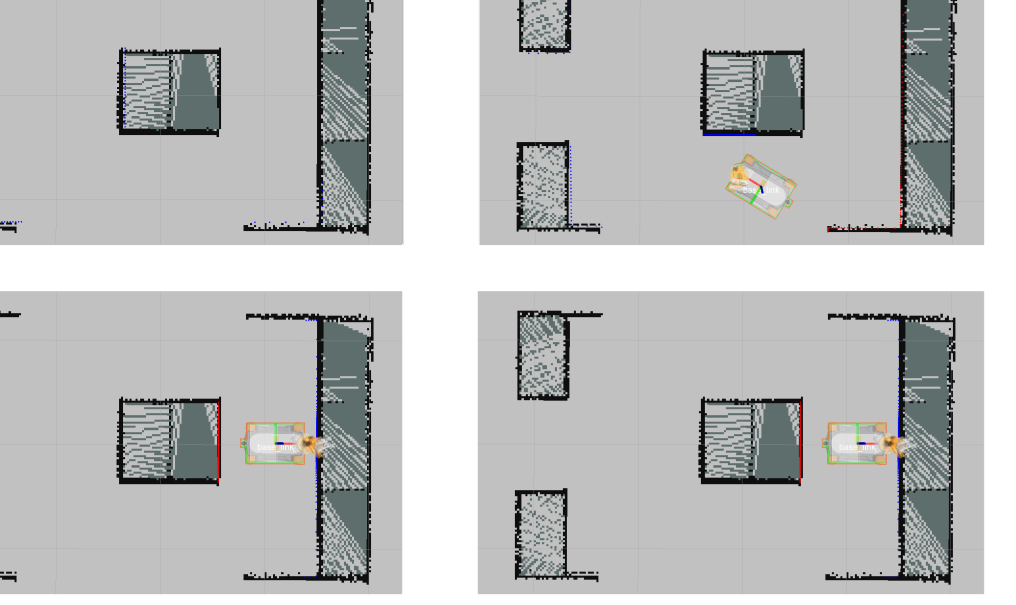
\includegraphics[scale=0.3]{images/base_absolute_exp.png}
\caption[Demonstrations to teach the youBot to move base to an absolute location]
{Demonstrations for teaching the robot to \textit{move} base
to an absolute pose in the workspace. The rows show the recorded start pose and the end pose. The 
columns show the different demonstrations}
\label{base absolute exp}
\end{figure}
\begin{figure}[htp]
\centering
\includegraphics[scale=0.5]{images/base_absolute_result.png}
\caption[Result : \textit{move} base absolute pose]{Results for \textit{ move}
base to an absolute pose. The x-axis denotes the number of demonstrations used
for learning. The y-axis denotes the method used for computing relevance.Each
box is marked with the selected template name. Green
color denotes the relavant template was successfully recommended}
\label{base absolute result}
\end{figure}


\FloatBarrier
\subsubsection{\textit{move} base relative pose to object }
In this experiment the youBot is taught to \textit{move} base to a relative
location in the workspace. The experiments consist of recording different start
and end poses of the robot in the workspace. First the robot is moved to any
arbitary position and the start pose is recorded then the robot is moved to the
intended final position which needs to be taught and the end pose is recorded.
The above steps are repeated till all the observations are recorded as
displayed in figure \href{base relative exp}.
As you can see the object was placed on different platform on each demonstrations.

This particular motion primitive
can be used as a part of the "basic manipulation test" task. In these task the
robot has to go near a platform containing an object. We ran the experiments
using different number of demonstrations and using both entropy and conditional
entropy for measuring relevance. The success of the experiments are shown in
figure \ref{base relative result}. The template describing the relative
distance between the base of youBot and the object was recommended as the most
relevant template from the demonstrations.

\begin{figure}[htp]
\centering
\includegraphics[scale=0.3]{images/base_relative_exp.png}
\caption[Demonstrations to teach the robot to move base to a relative location]
{Demonstrations for teaching the robot to \textit{move} base
to a relative pose in the workspace. The rows show the recorded start pose and the end pose. The 
columns show the different demonstrations}
\label{base relative exp}
\end{figure}
\begin{figure}[htp]
\centering
\includegraphics[scale=0.5]{images/base_relative_result.png}
\caption[Result : \textit{move} base relative pose to object  ]{Results for \textit{ move} base to a relative pose. The x-axis denotes the 
number of demonstrations used for learning. The y-axis denotes the method used for 
computing relevance.Each
box is marked with the selected template name. Green color denotes the relavant template was successfully recommended}
\label{base relative result}
\end{figure}

\FloatBarrier
\subsubsection{\textit{move} arm absolute pose}
In this experiment the youBot is
taught to \textit{move} arm to an absolute pose.
The experiments consist of recording different start and end poses of the robot arm. 
First the robot arm is moved to any arbitary position and the start pose is recorded then 
the robot arm is moved to the intended final position which needs to be taught and the end 
pose is recorded. The above steps are repeated till all the observations are recorded as shown in figure \ref{arm absolute exp}


This particular motion primitive can be used as a part of the "basic manipulation test" task. In these
task the robot has to be taught the "look platform" pose for looking at the platform.
We ran the experiments using different number of demonstrations and using both entropy 
and conditional entropy for measuring relevance. The success of the experiments are 
shown in figure \ref{arm absolute result}. 
The template describing the joint angles of the arm was recommended as the most
relevant template from the demonstrations.
\begin{figure}[htp]
\centering
\includegraphics[scale=0.6]{images/arm_absolute_exp.png}
\caption[Demonstrations to teach the robot to move arm to an absolute location ]
{Demonstrations for teaching the robot to \textit{move} arm
to an absolute pose in the workspace. The rows show the recorded start pose and the end pose. The 
columns show the different demonstrations}
\label{arm absolute exp}
\end{figure}

\begin{figure}[htp]
\centering
\includegraphics[scale=0.5]{images/arm_absolute_result.png}
\caption[Result : \textit{move} arm absolute pose]{Results of \textit{ move} arm to an absolute pose. The x-axis denotes the 
number of demonstrations used for learning. The y-axis denotes the method used for 
computing relevance.Each
box is marked with the selected template name. Green color denotes the relavant template was successfully recommended}
\label{arm absolute result}
\end{figure}


\FloatBarrier
\subsubsection{\textit{move} arm relative pose to object}
In this experiment the youBot is
taught to \textit{move} arm to a relative pose to an external object.
The experiments consist of recording different start and end poses of the robot arm. 
First the robot arm is moved to any arbitary position and the start pose is recorded then 
the robot arm is moved to the intended final position which needs to be taught and the end 
pose is recorded. The above steps are repeated till all the observations are recorded.


This particular motion primitive can be used as a part of the "precision placement test" task. In these
task the robot has to be place the object precisely inside a cavity. So the robot has to be taught to place
the object relative to placement cavity.
We ran the experiments using different number of demonstrations and using both entropy 
and conditional entropy for measuring relevance. The success of the experiments are 
shown in figure \ref{arm relative results}. 
The template describing the relative distance between the tooltip and the object  was recommended as the most
relevant template from the demonstrations.
\begin{figure}[htp]
\centering
\includegraphics[scale=0.5]{images/arm_relative_result.png}
\caption[Result : \textit{move} arm relative pose to object]{Results of \textit{ move} arm to an relative pose. The x-axis denotes the 
number of demonstrations used for learning. The y-axis denotes the method used for 
computing relevance.Each
box is marked with the selected template name. Green color denotes the relavant template was successfully recommended}
\label{arm relative results}
\end{figure}

\FloatBarrier
\subsubsection{\acrlong{ndcg} based evaluation}
The following section has the evalutaion based on the \acrshort{ndcg}@1 
and \acrshort{ndcg}@2 metrics.
For evalutation the templates in the knowledge base was labeled on a 3 point
likert scale.
We ran the algorithm using entropy as out relevance function.

Figure \ref{ndcg 1} shows the \acrshort{ndcg}@1 plots for different number of 
demonstrations. Its clear that with 3 demonstrations the algorithm is able to
predict the expected template in all the experiments.

Figure \ref{ndcg 3} shows the \acrshort{ndcg}@3 plots for different number of 
demonstrations. We can observe that with increasing number of demonstrations the
quality of the recommendations are improving. With 3 demonstrations the 
quality of the recommendations is well above 60\% for all the experiments.

\begin{figure}[htp]
\centering
\includegraphics[scale=0.4]{images/nDCG@1.png}
\caption[nDCG@1 score based comparison]{nDCG@1 values for the experiments conducted.
The y-axis is the nDCG@1 score. The x-axis consist of groups of 2 bars arranged
as experiments conducted. Each bar in the experiment corresponds to the number
of demonstration used to make the recommendations. }
\label{ndcg 1}
\end{figure}

\begin{figure}[htp]
\centering
\includegraphics[scale=0.4]{images/nDCG@3.png}
\caption[nDCG@3 score based comparison]{nDCG@3 values for the experiments conducted.
The y-axis is the nDCG@3 score. The x-axis consist of groups of 4 bars arranged
in the sequntial order of the  experiments conducted. Each bar in the experiment corresponds to the number
of demonstration used to make the recommendations. }
\label{ndcg 3}
\end{figure}
\FloatBarrier
\subsection{Discussions}
The proposed approach recommends the relevant features with higher probability.
It has been observed that using entropy based likehood measuring method we could
achieve a success rate of 100\% using just 3 demonstrations.
The higher success rate ensure that the entropy based method is a reliable way to
determine the relevant features.
While using the conditional entropy based relevance measuring method we could 
only achieve a success rate of 62.8\%. 
The lower success rate means that conditional entropy cannot be used for recommending 
the relevant features.

